\section{Implementación y programación}\label{sec:implemetacion_y_programacion}

En esta sección vamos a explicar algunos de los detalles de implementación de aquellos componentes que creemos que es
interesante que sean introducidos.

\subsection*{Componente \textit{Generator}}

\subsubsection*{PDF To Text Processor}

Cómo introducimos en la sección~\ref{sec:diseno_del_sistema} Diseño del sistema, este procesador es responsable de
convertir un fichero \textit{PDF} en un fragmento de texto plano.

Tal y como puede verse en el extracto de código de la figura~\ref{fig:chapter_4.4.pdf_to_text_processor}, el procesador
\textit{PDF To Text Processor} es simplemente un envoltorio para la herramienta de línea de comandos
\textit{Pdf To Text}.

\begin{figure}[ht]
    \begin{center}
        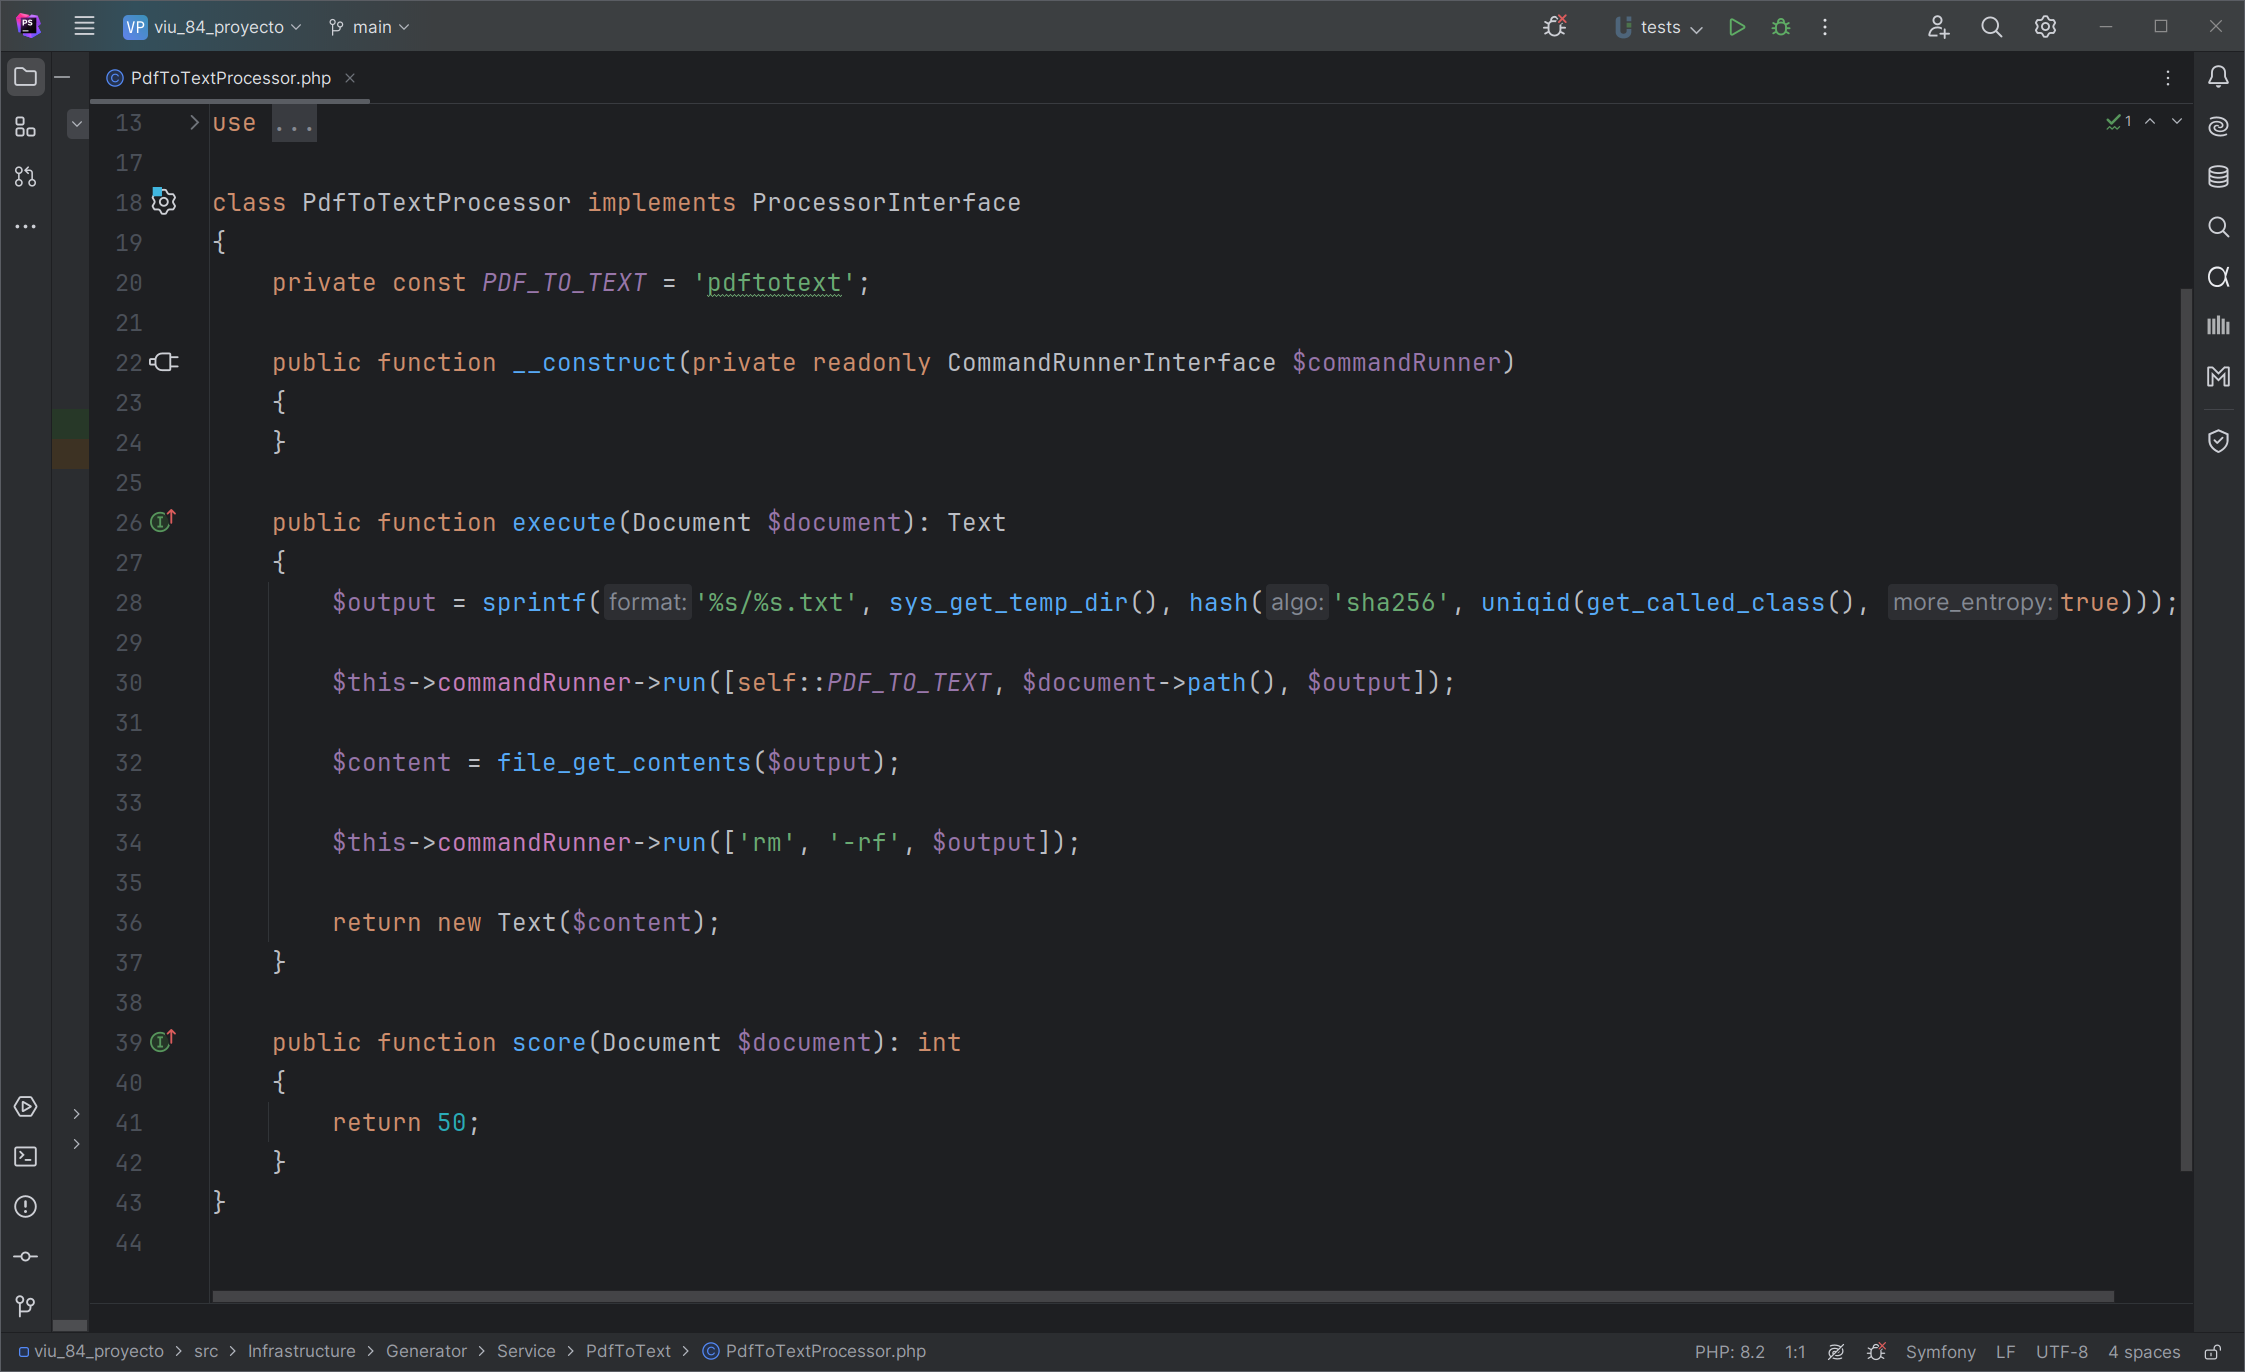
\includegraphics[width=\textwidth]{./chapter/4/images/chapter_4.4.pdf_to_text_processor}
        \caption{Captura del código fuente del procesador \textit{PDF To Text Processor}}
        \label{fig:chapter_4.4.pdf_to_text_processor}
    \end{center}
\end{figure}

En la figura~\ref{fig:chapter_4.4.generator_component_pdf_to_text_processor} puede verse un esquema de este
comportamiento: el motor envía el documento \textit{PDF} al procesador, este a su vez lo envía a \textit{PDF To Text}
el cual genera un fichero de texto plano.
Finalmente, el procesador extrae el contenido de ese fichero y lo envía de vuelta al motor, donde comenzó todo.

\begin{figure}[ht]
    \begin{center}
        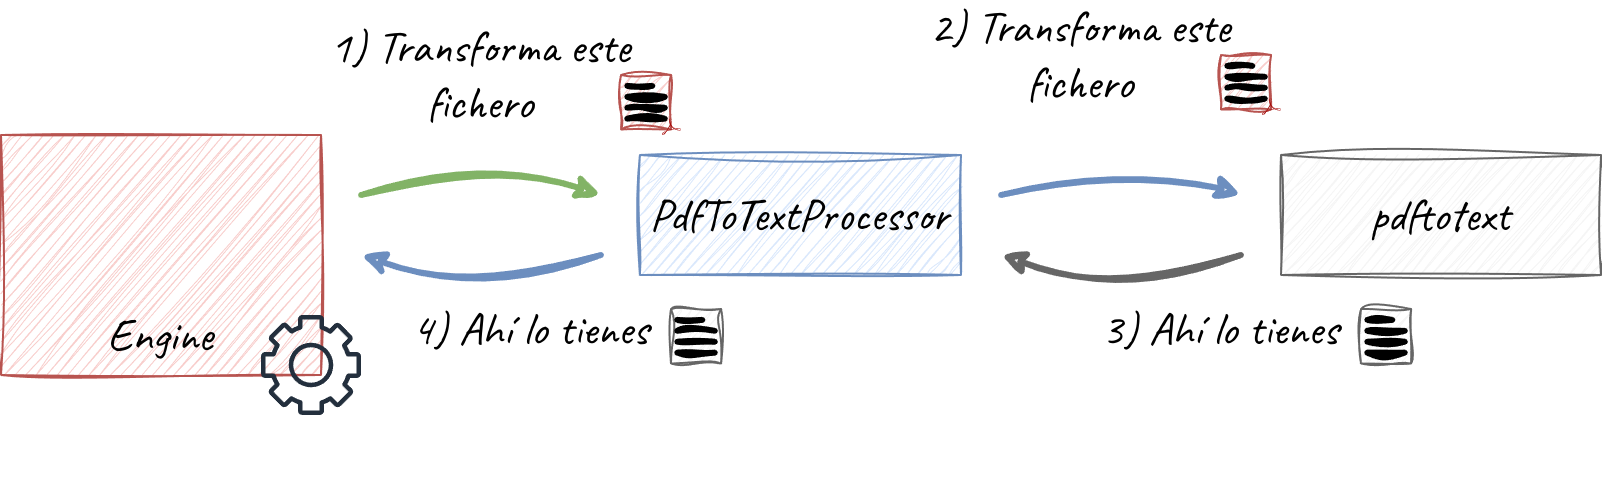
\includegraphics[width=\textwidth]{./chapter/4/images/chapter_4.4.generator_component_pdf_to_text_processor}
        \caption{Esquema de comunicación con la herramienta de la capa de infraestructura pdftotext}
        \label{fig:chapter_4.4.generator_component_pdf_to_text_processor}
    \end{center}
\end{figure}

\subsection*{Componente \textit{Reader}}

De este componente queremos destacar los siguientes elementos, el \textit{Residential Lease Agreement Processor} y el
\textit{Vehicle Sale And Purchase Agreement Processor} responsables de extraer la información de los contratos de
alquiler de vivienda entre particulares y la compraventa de vehículos entre particulares respectivamente.

\subsubsection*{Residential Lease Agreement Processor}

Cómo introducimos en la sección~\ref{sec:diseno_del_sistema} Diseño del sistema, este procesador es responsable de
transformar el texto de un contrato de arrendamiento de vivienda entre particulares en un objeto con sus datos
fundamentales.

La implementación de este procesador es muy similar a la que hemos visto en el \textit{PDF To Text Processor}, por lo
que no vamos a incluir ni el código ni el esquema con la comunicación.

Simplemente, indicaremos que se trata de enviar peticiones sobre un documento que previamente hemos convertido en texto
plano a un sistema que lo pueda procesar, en este caso nos hemos decantado por \textit{ChatGPT 4 Turbo}~
\cite{url_openai_gpt4}

Si merece la pena profundizar en las características de las peticiones que se envían.
La parte más compleja de estos componentes es encontrar un \textit{prompt} o entrada lo suficientemente precisa para que
genere una respuesta que pueda ser utilizada a continuación.

Para encontrar una entrada suficientemente precisa, utilizamos dos técnicas:

La primera \textit{Few-shot Prompting}~\cite{article_few_shot_prompting} es una técnica en la cual se proporcionan
al modelo ejemplos de entrada y salida para que aprenda el patrón específico.
Por ejemplo para una persona se indica: \textit{\{"name": "John", "surname": "Doe", "number": "12345678 A"\}}.

La segunda técnica es el \textit{Format-based Prompting}~\cite{article_format_based_prompting}, una técnica en la
cual se estructura el prompt para guiar al modelo a generar respuestas en un formato específico, como \textit{JSON},
listas o tablas, las cuales pueden ser luego fácilmente parseadas.

El primer intento de implementación se trató que el modelo respondiera con un \textit{XML}.
Sin embargo, \textit{ChatGPT 4} tiene limitaciones para trabajar con documentos \textit{XML}, por lo que la
implementación final se realizó utilizando modelos \textit{JSON}.

Todo esto puede verse en el ejemplo de código que aparece en la
figura~\ref{fig:chapter_4.4.residential_lease_agreement_processor}, donde se muestra el código del método que define el
\textit{prompt}.

\begin{figure}[ht]
    \begin{center}
        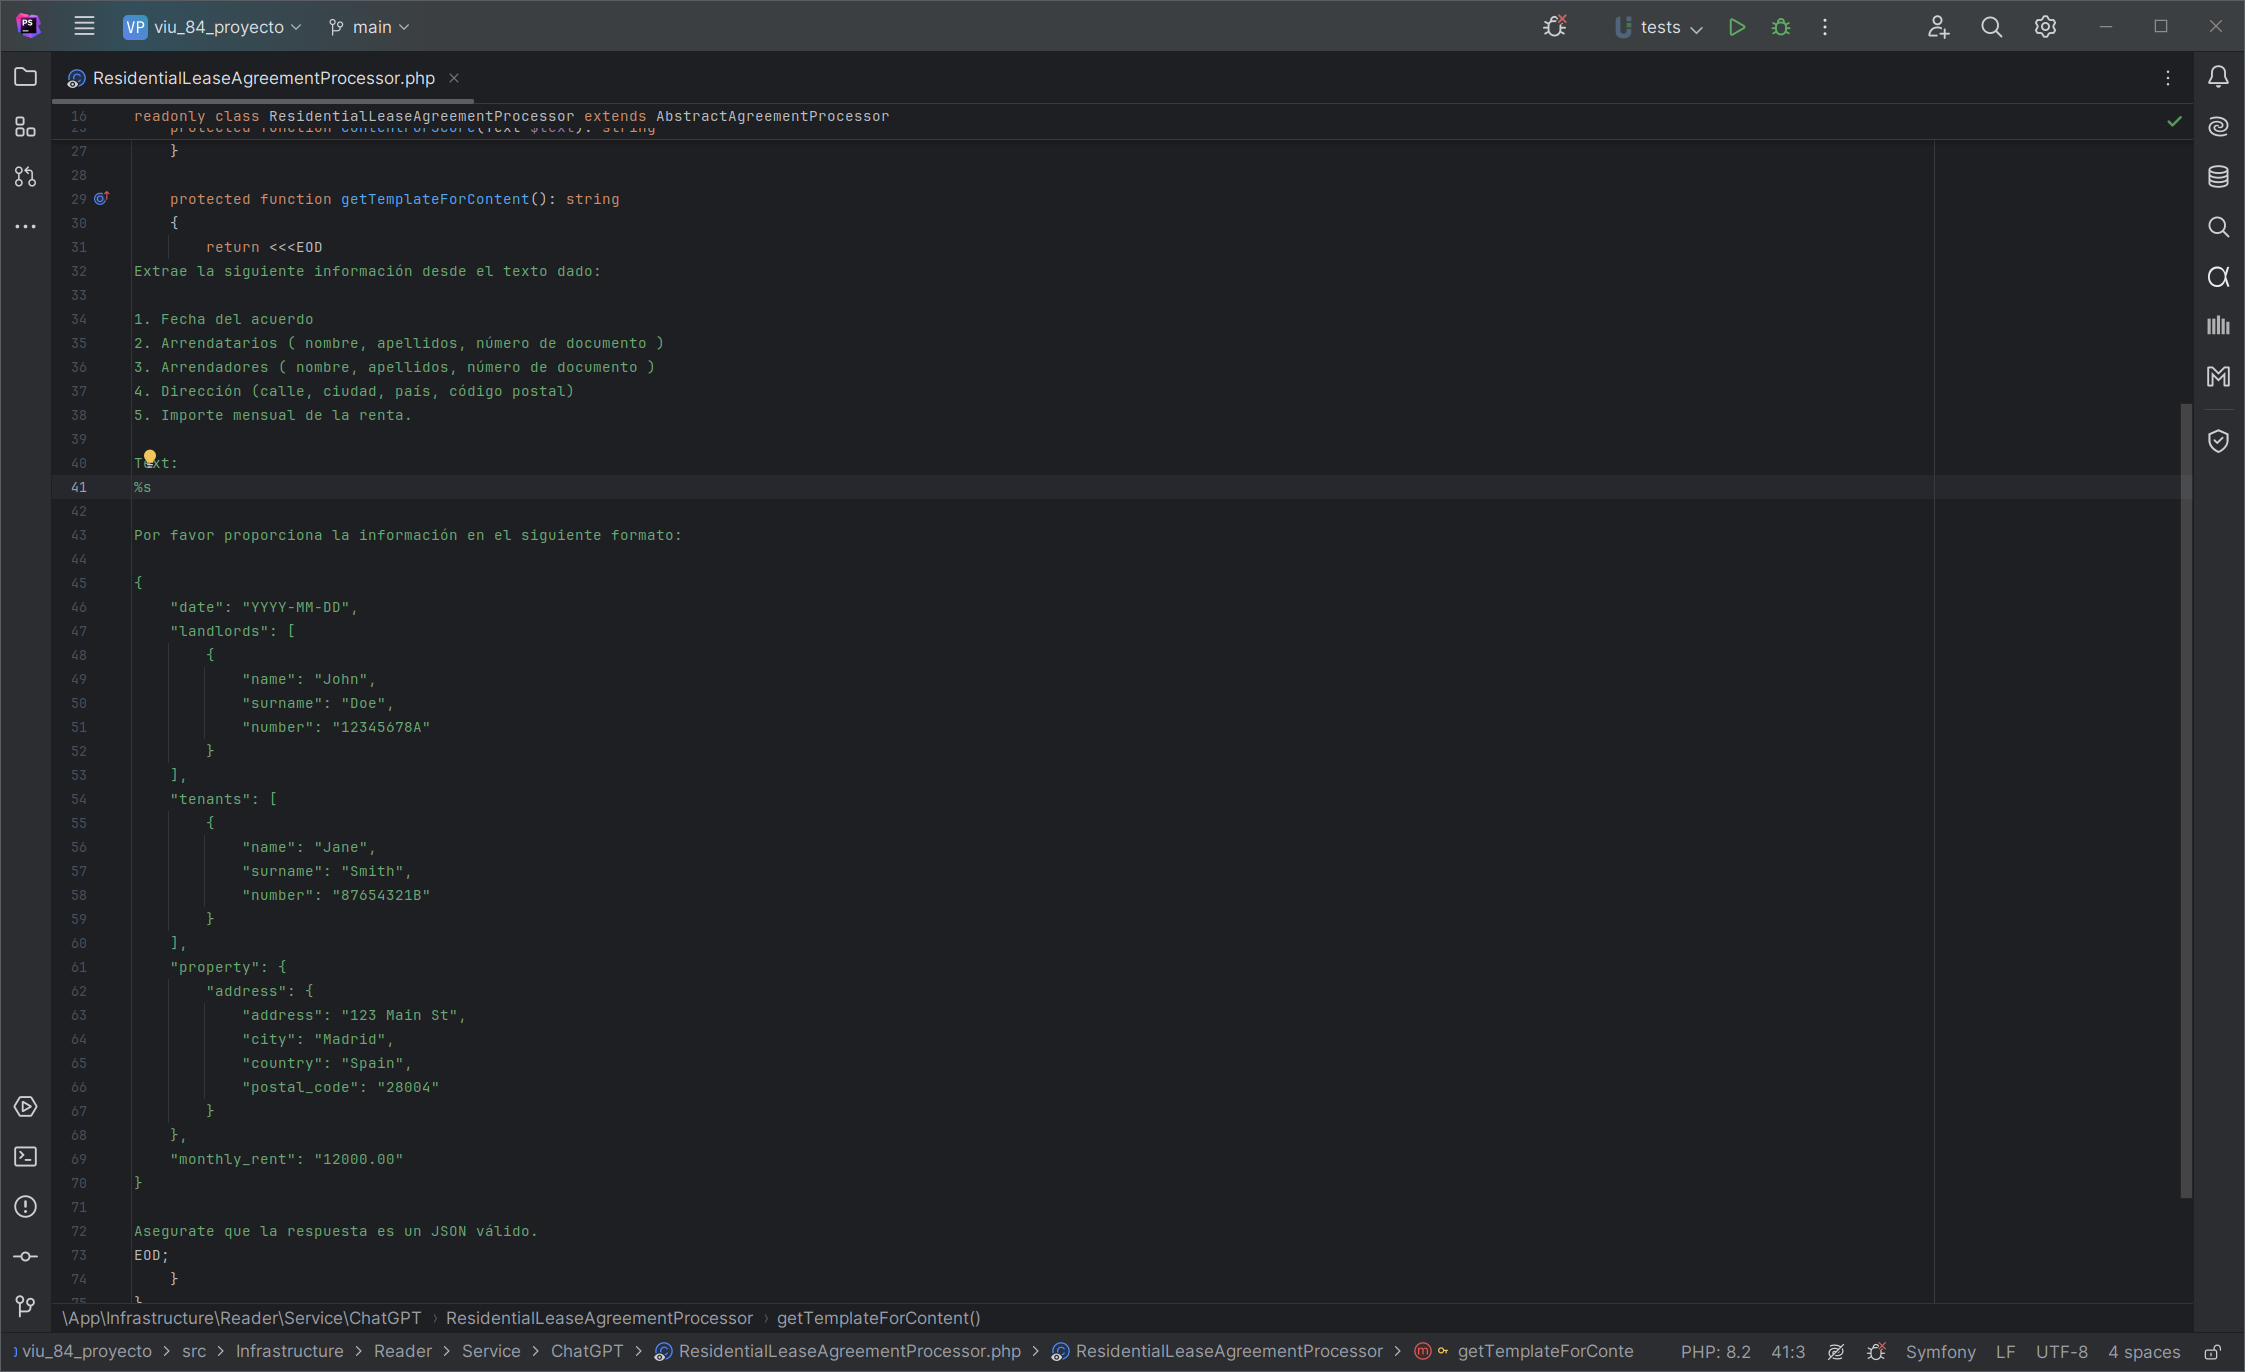
\includegraphics[width=\textwidth]{./chapter/4/images/chapter_4.4.residential_lease_agreement_processor}
        \caption{Captura del código fuente del procesador \textit{Residential Lease Agreement Processor}}
        \label{fig:chapter_4.4.residential_lease_agreement_processor}
    \end{center}
\end{figure}

Una vez que se obtiene la respuesta en formato \textit{JSON}, tan solo es necesario des-serializar para convertirlo
en un objeto del tipo indicado, en este caso un \textit{Residential Lease Agreement} que como puede verse en la
figura~\ref{fig:chapter_4.4.residential_agreement} que aparece contiene los tipos de datos esperados para un contrato de
arrendamiento de vivienda entre particulares.

\begin{figure}[ht]
    \begin{center}
        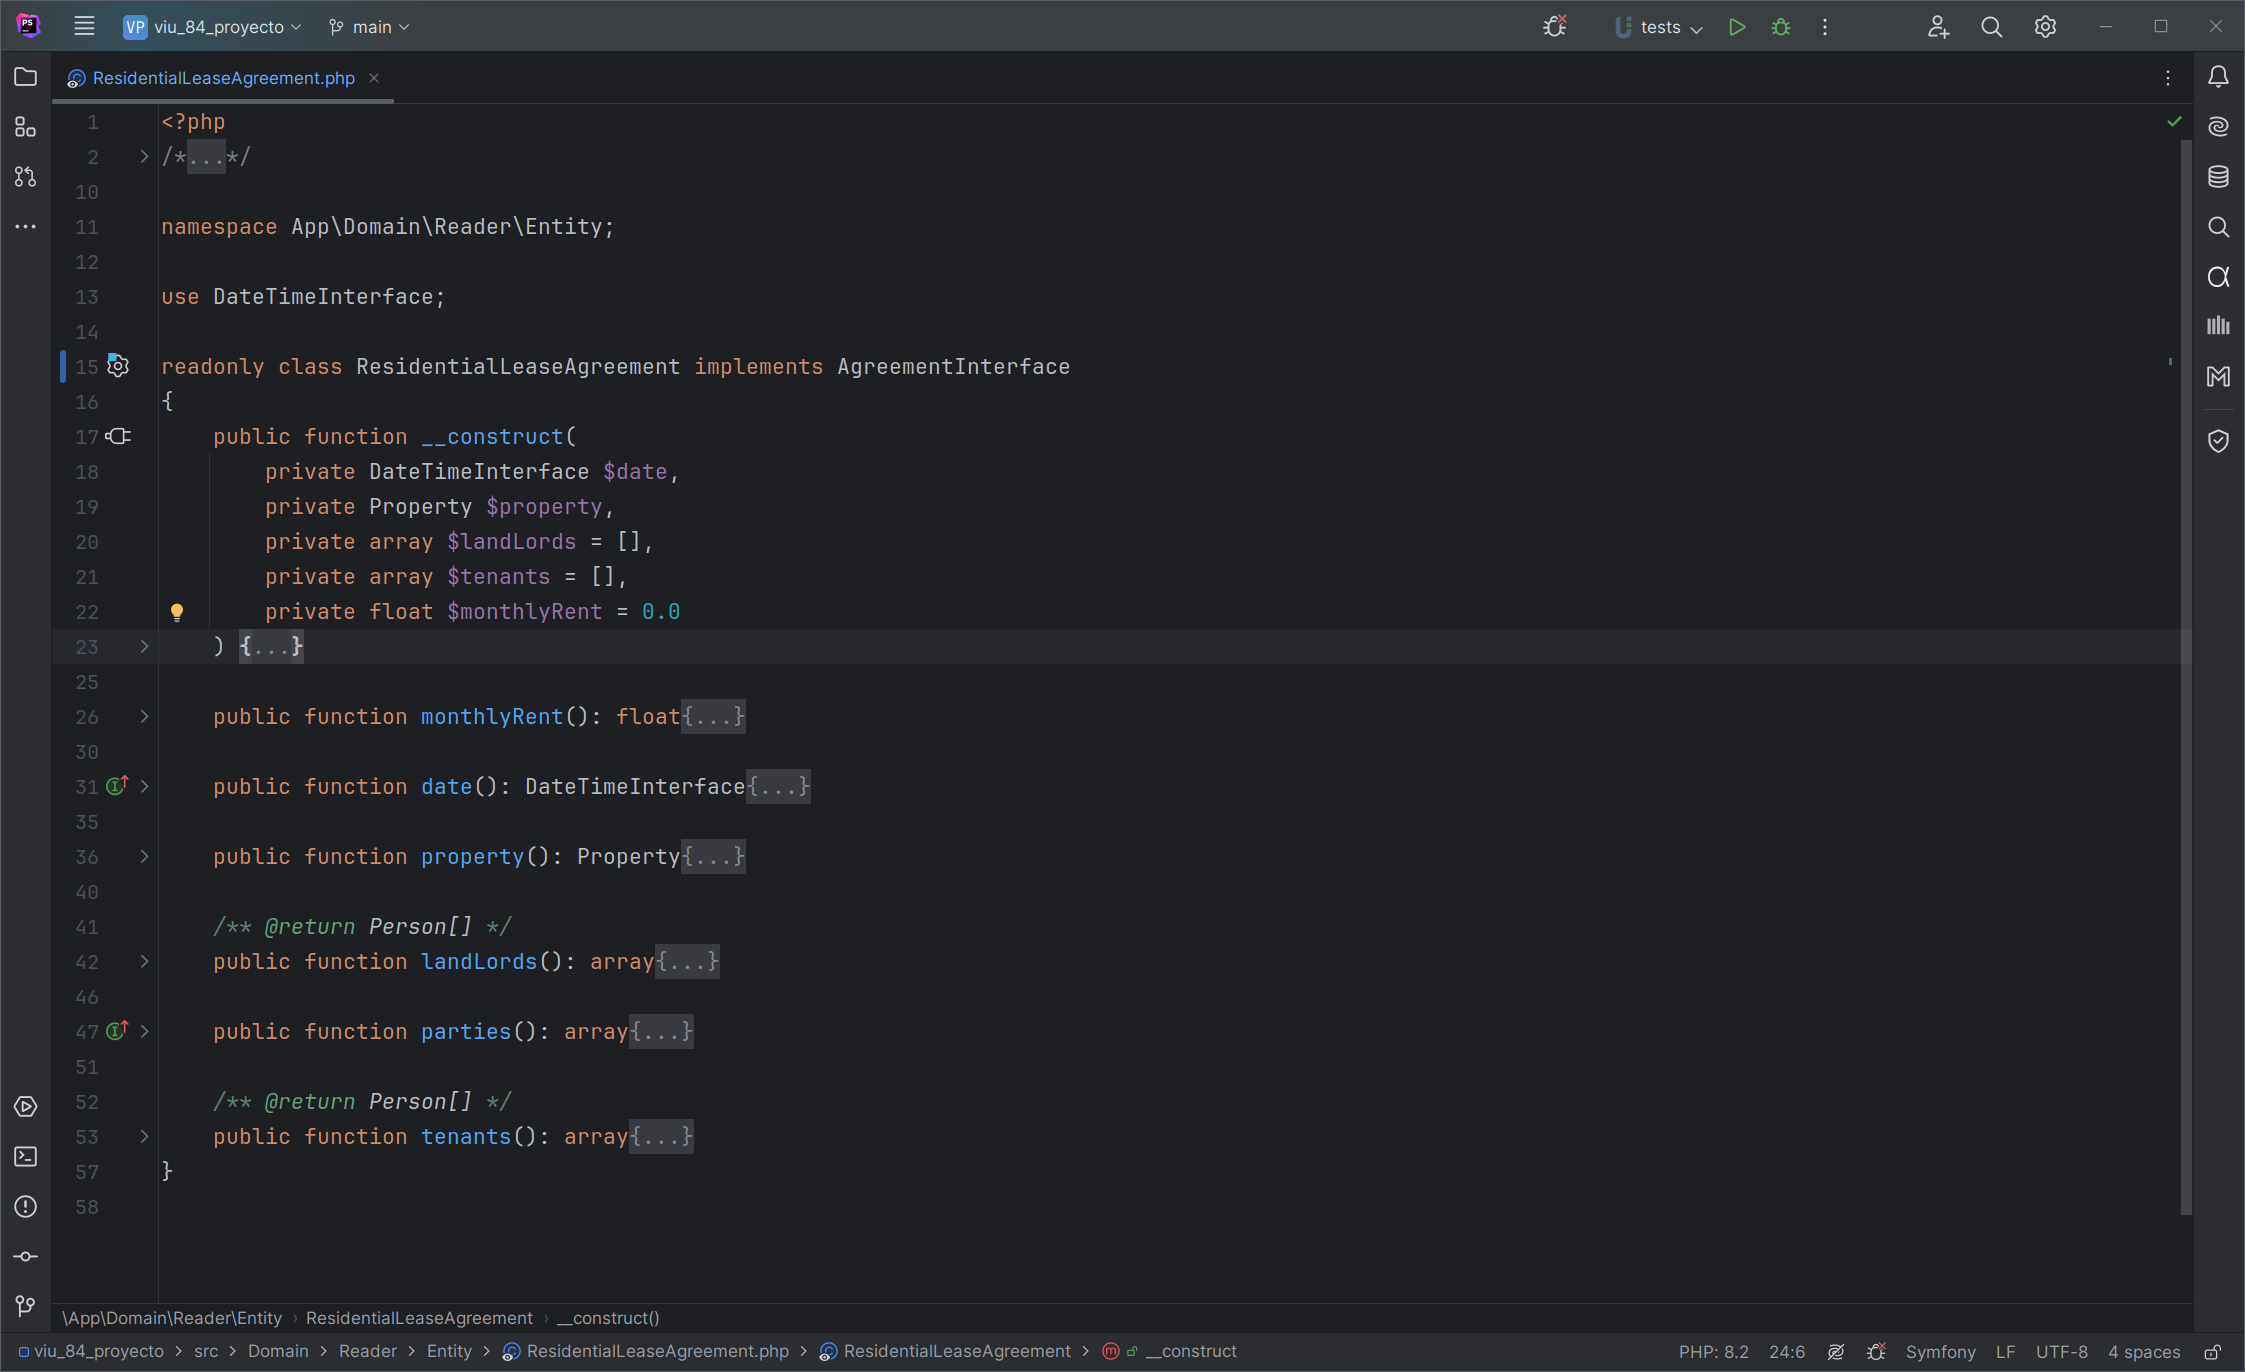
\includegraphics[width=\textwidth]{./chapter/4/images/chapter_4.4.residential_lease_agreement}
        \caption{Captura del código fuente de la entidad \textit{Residential Lease Agreement}}
        \label{fig:chapter_4.4.residential_agreement}
    \end{center}
\end{figure}

La \textit{API} de \textit{ChatGPT 4} presenta dos problemas: es lenta y cuesta dinero.
Los tiempos de respuesta pueden variar dependiendo del tipo de documento y del estado de la api.
Los costes también pueden variar dependiendo del tipo de documento y del precio de la api en ese
momento~\cite{url_openai_api_pricing}.

A continuación una tabla calculada con el promedio de 100 peticiones para el documento \textit{001/001.pdf}.

\begin{table}[h]
    \renewcommand{\arraystretch}{1.5}
    \setlength{\tabcolsep}{10pt}
    \begin{tabular}{p{0.60\textwidth} p{0.30\textwidth}}
        \toprule
        \textbf{Nombre}              & \textbf{Valor} \\
        \midrule
        Total peticiones             & 3              \\
        Tiempo total                 & 6.74 segundos  \\
        Total \textit{input tokens}  & ~6643          \\
        Total \textit{output tokens} & ~159           \\
        Precio total                 & ~0.07 euros    \\
        \bottomrule
    \end{tabular}
    \caption{Resumen de los resultados de la ejecución procesador \textit{Residential Lease Agreement Processor}}
    \label{tab:residential_lease_processor}
\end{table}

Un token en un modelo \textit{ChatGPT} es una unidad básica de texto que puede ser una palabra, parte de una palabra
o un carácter de puntuación.

Aunque los modelos \textit{ChatGPT} tienen limitaciones en cuanto al tamaño máximo del contexto, como se muestra en la
tabla~\ref{tab:chat_gpt_limits}, estas limitaciones no afectan la ejecución de este procesador~\cite{url_openai_models}.

En el post procesador \textit{Word Limit Post Processor}, descrito en la sección \ref{sec:diseno_del_sistema} Diseño
del sistema, se asume que la información relevante para este caso de uso se encuentra dentro de las primeras 1000
palabras de cada documento, truncándose cualquier información que exceda este límite.

Estimando un promedio de 1.3 tokens por palabra, esto se mantiene dentro de los límites permitidos por los modelos más
recientes.

\begin{table}[h]
    \renewcommand{\arraystretch}{1.5}
    \setlength{\tabcolsep}{10pt}
    \begin{tabular}{p{0.70\textwidth} >{\raggedleft\arraybackslash}p{0.20\textwidth}}
        \toprule
        \textbf{Modelo} & \textbf{Tokens por contexto} \\
        \midrule
        GPT-4 turbo     & 128,000 tokens               \\
        GPT-4           & 8,192 tokens                 \\
        GPT-3.5 turbo   & 16,385 tokens                \\
        \bottomrule
    \end{tabular}
    \caption{Límite de tokens por contexto para los modelos más recientes de \textit{ChatGPT}}
    \label{tab:chat_gpt_limits}
\end{table}

Cabe mencionar que durante la fase de desarrollo de este proyecto se repitieron continuamente los mismos documentos,
en un ciclo de prueba y error.
Por lo que tanto para acelerar los tiempos de ejecución como para reducir los costes se hizo recomendable implementar un
sistema de caché.

El sistema de caché genera un hash para cada petición y guarda la respuesta, durante un tiempo limitado.
Si se repite una misma petición recupera la respuesta de la caché, por lo que la respuesta es prácticamente
instantánea y sin ningún coste adicional.

\subsubsection*{Vehicle Sale And Purchase Agreement Processor}

Este procesador es responsable de transformar el texto de un contrato de compraventa de vehículo entre particulares en
un objeto con sus datos fundamentales.

Este procesador funciona de forma tan similar al procesador anterior que no será necesario entrar en nuevos detalles
con respecto a su funcionamiento, hasta el punto de que en el momento del desarrollo fue evidente que podrían
compartir una parte muy importante del código, simplemente cambiando ligeramente las peticiones que se debían realizar.

\subsection*{Registros}\label{subsec:logs}

El registro de \textit{logs} es una parte crucial del monitoreo y mantenimiento de cualquier aplicación.
En proyectos de este tipo, por la cantidad de pequeños componentes y por interactuar con elementos de infraestructura
externos, se hace necesario contar con un buen sistema de registro de logs.

En este proyecto, se ha implementado un sistema de registros utilizando \textbf{Monolog}, una biblioteca de registro
para PHP.

Se han configurado tres canales.

\begin{itemize}
    \item Generator: para los logs del componente generator.
    \item Reader: para los logs del componente reader.
    \item Http-Client: para el componente que realiza las peticiones HTTP.
\end{itemize}

Un canal es la forma en la que monolog, agrupa un conjunto de información para poder filtrar y procesar adecuadamente.
Además, los logs se almacenan en dos ficheros y formatos diferentes:

\begin{itemize}
    \item \textbf{Monolog format}, es el formato estándar de ficheros de log generados por esta biblioteca.
    \item \textbf{Logstash format}, es el estándar de la herramienta \textbf{Monolog}.
\end{itemize}

El formato \textbf{Monolog format} está indicado para entornos de desarrollo o proyectos de pequeña envergadura.
Siempre que estos ficheros no sean demasiado grandes, se pueden trabajar a través de herramientas de línea de comandos
como \textbf{grep} o \textbf{awk}.

El formato \textbf{Logstash format} es adecuado para ser procesado por un sistema compuesto por
\textbf{Elasticsearch}, \textbf{Logstash} y \textbf{Kibana} (ELK).
Este formato está indicado en entornos de producción, donde la monitorización de los logs sea una tarea relevante.

En la figura~\ref{fig:chapter_4.4.logs_overview} puede verse un esquema de este comportamiento.

\begin{figure}[ht]
    \begin{center}
        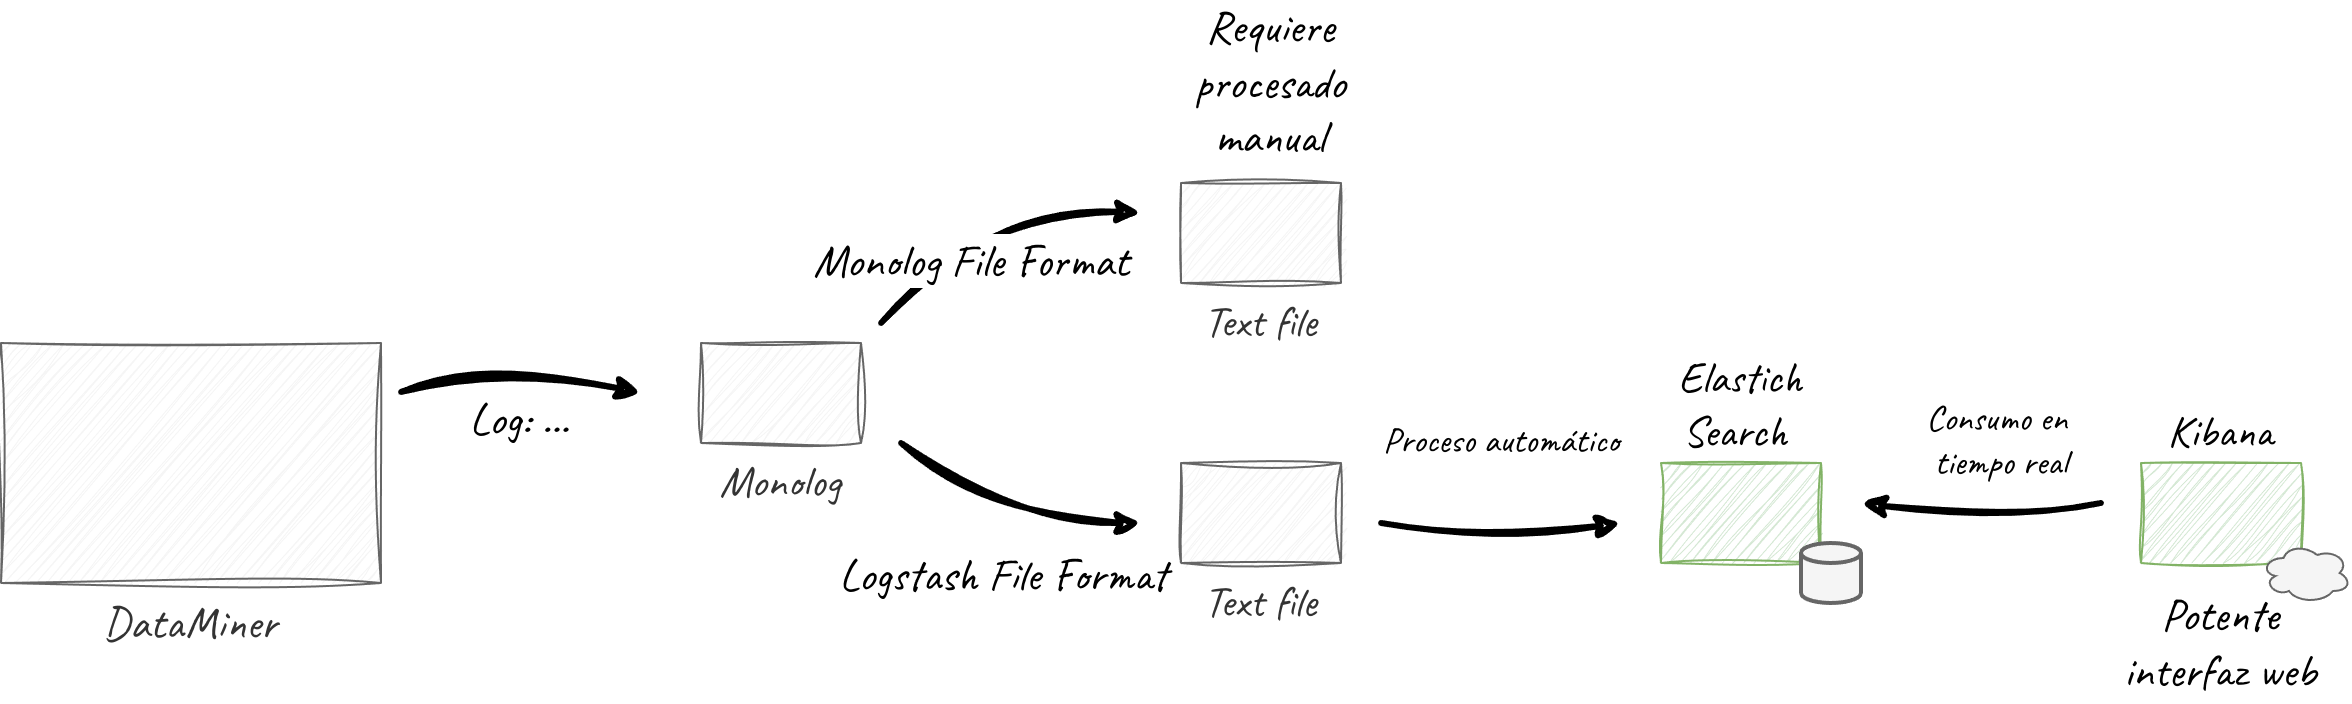
\includegraphics[width=\textwidth]{./chapter/4/images/chapter_4.4.logs_overview}
        \caption{Esquema del sistema de procesamiento de logs}
        \label{fig:chapter_4.4.logs_overview}
    \end{center}
\end{figure}